\appendix
\begin{center}
  {\zihao{4}\bfseries 附录}
\end{center}

\section{输入插值留出检验}

图\ref{fig:input-holdout}(a)--(c)比较留出观测与两种插值重建，(d)--(f)给出逐时刻残差、RMSE、MAE和最不利留出点，(g)再用持续值RMSE归一化三种不同量纲的输入。线性插值相对持续值基线分别降低环境温度、环境含湿量和半径RMSE约35.4\%、36.6\%和91.8\%；PCHIP没有稳定优势。留出点来自原观测时段，故该检验不评价4 h后的环境延拓。

\begin{figure}[H]
  \centering
  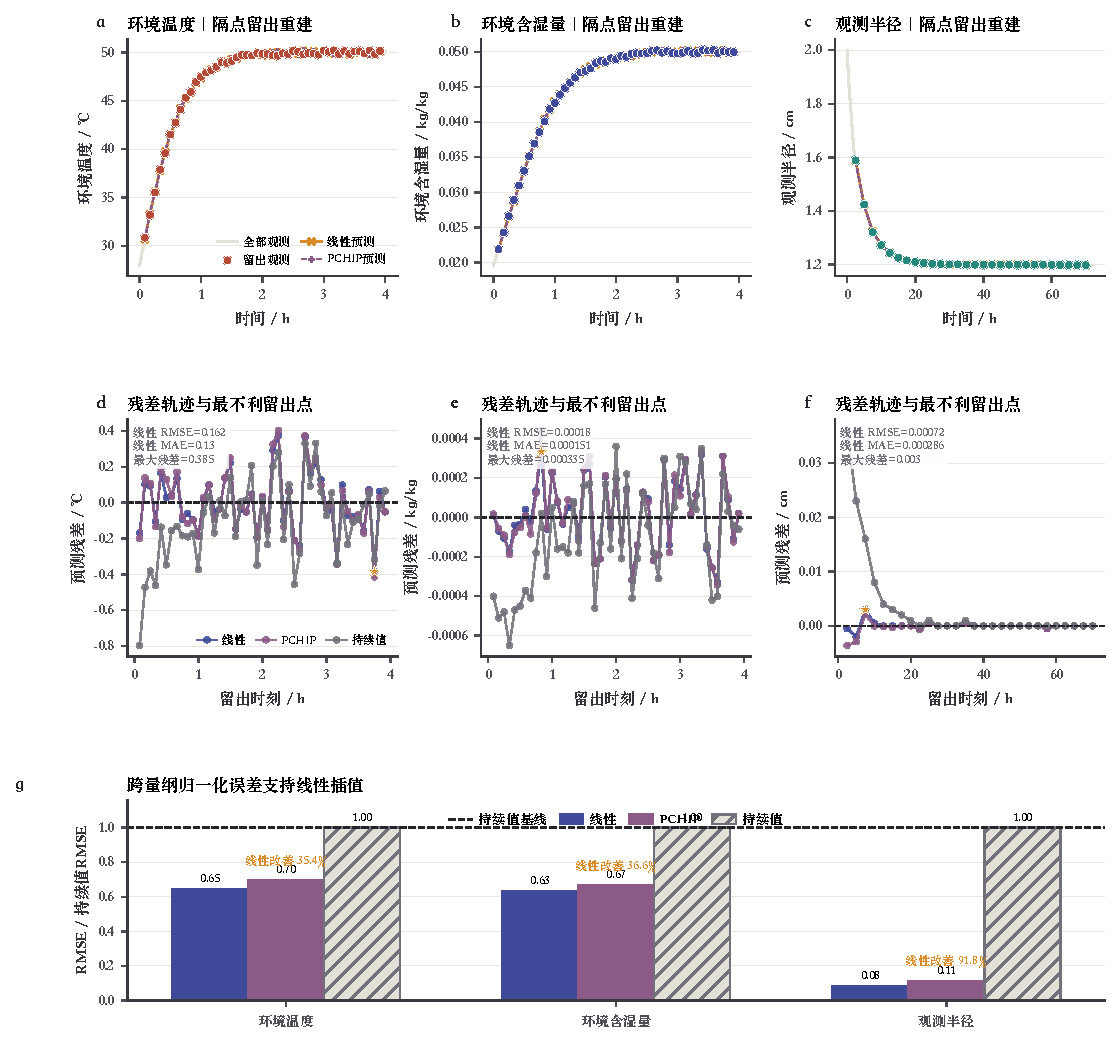
\includegraphics[width=\textwidth]{figures/figS01_input_holdout.pdf}
  \caption{输入插值留出检验}
  \label{fig:input-holdout}
\end{figure}

\section{端面假设条件对照}

二维轴对称对照设置两种情景：E0端面绝热、不透湿；E1端面与侧面采用相同$h$、$h_m$及环境条件。每个E1结果都与同径向网格、同容差、同最大步长的E0配对，避免把粗二维离散误差误算为端面效应。图\ref{fig:endface-assessment}(a)(b)给出3 h二维场差，(c)把径向最大差投影为距端面距离的衰减曲线，(d)(e)比较整根平均量与不同输出尺度，(f)检查配对效应在细化情景下是否保持同一量级。因此，端面影响不能只由面积比例判断，也不能用单一中截面指标代表整根药材。

\begin{figure}[H]
  \centering
  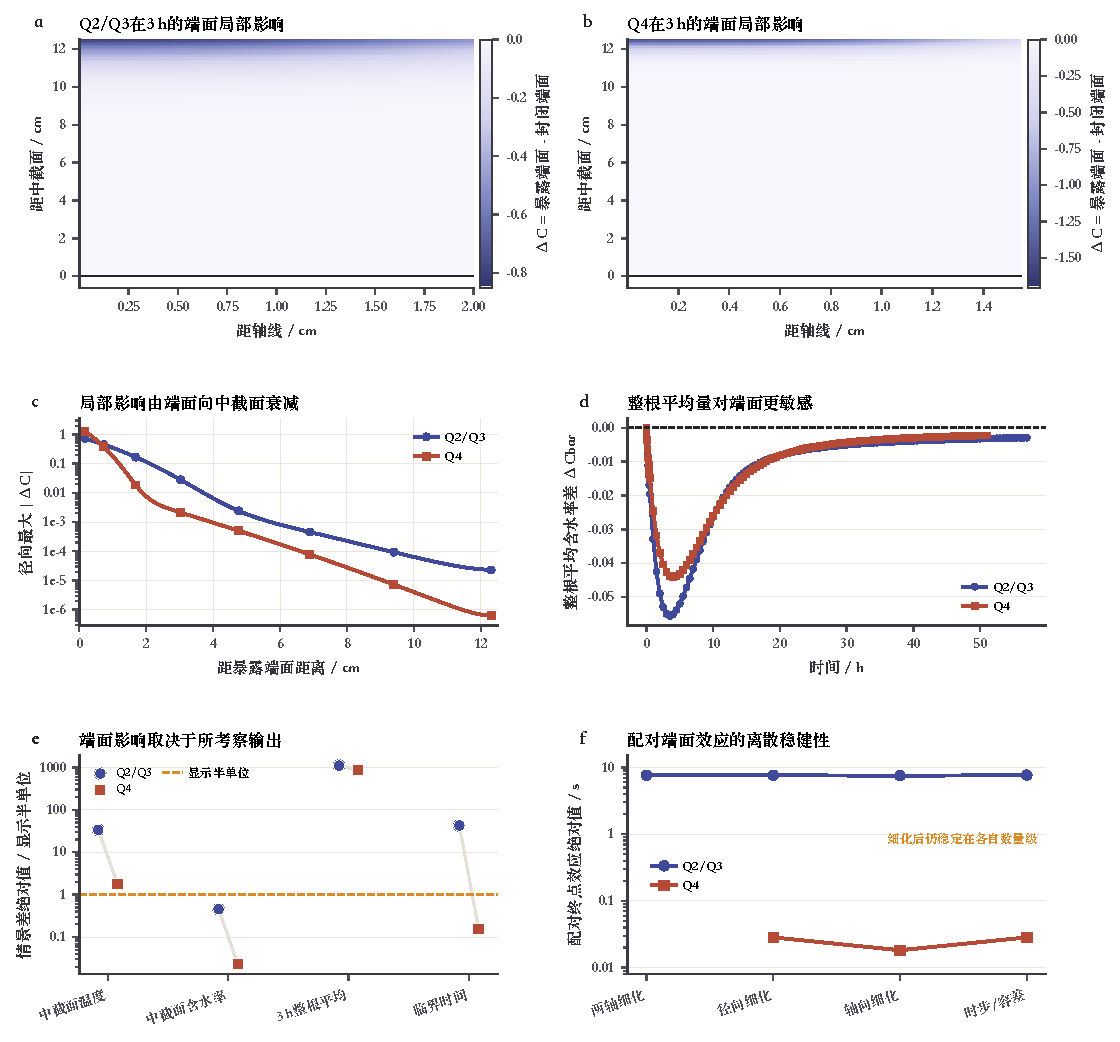
\includegraphics[width=\textwidth]{figures/figS02_endface_assessment.pdf}
  \caption{端面假设条件对照}
  \label{fig:endface-assessment}
\end{figure}

端面暴露的影响主要集中在靠近两端的局部区域，中截面差异明显较小。配对细化后，问题三临界时间约提前$7.49$ s，问题四约提前$0.0284$ s；问题二前三小时的中截面温度最大差约$0.0017\ ^\circ\mathrm C$。这说明端面假设对本文一维中截面结论影响有限，但整根平均量和端部局部场仍需在实际应用中单独校准。

\section{主要程序与结果文件}

\begin{table}[H]
  \caption{支撑文件说明}
  \label{tab:support-files}
  \centering
  \begin{tabularx}{0.96\textwidth}{lX}
    \toprule
    文件或目录 & 说明 \\
    \midrule
    \texttt{scripts/question1.py}--\texttt{question4.py} & 四问主求解入口 \\
    \texttt{src/} & 物性、边界、有限体积离散、重建与求解模块 \\
    \texttt{config/model\_config.json} & 几何、物性、边界、时间线及输入路径配置 \\
    \texttt{validation/} & 解析基线、独立有限元、收敛、守恒、端面与反例检验 \\
    \texttt{results/submission/result1.xlsx}--\texttt{result4.xlsx} & 按题目模板另存的最终结果文件，原始附件未覆盖 \\
    \texttt{figures/} & 论文图的PDF、SVG及600 dpi位图版本 \\
    \texttt{reports/final\_result\_validation.md} & 工作簿与主结果的最终验证记录 \\
    \texttt{AI工具使用详情.pdf} & 工具名称、使用过程及人工复核说明，提交前由参赛队确认 \\
    \bottomrule
  \end{tabularx}
\end{table}

\section{核心求解源程序}

下列程序包括问题一至问题四的主入口及其全部公共求解依赖。程序从项目根目录读取
\texttt{config/model\_config.json}。生产结果所用参数为：
\begin{itemize}[nosep,leftmargin=2em]
  \item 问题一：$N=1280$，表面加密指数为2，\texttt{rtol=1e-10}，最大步长1 s；
  \item 问题二：$N=1280$，表面加密指数为2，\texttt{rtol=1e-10}，最大步长2 s；
  \item 问题三：父轨迹为\texttt{q2\_final}，\texttt{rtol=1e-10}，最大步长30 s；
  \item 问题四：$N=1280$，表面加密指数为2，\texttt{rtol=1e-10}，最大步长30 s。
\end{itemize}
导出、绘图及全部验证程序随支撑材料一并提交，文件类别已列于表\ref{tab:support-files}。

\lstset{
  style=Python,
  basicstyle=\zihao{-6}\ttfamily,
  numberstyle=\zihao{-6}\ttfamily,
  frame=single,
  breaklines=true,
  breakatwhitespace=false,
  columns=fullflexible,
  keepspaces=true,
  tabsize=4,
  keywordstyle=\color{blue}\bfseries
}

\subsection{四问主程序}

\noindent\textbf{文件：}\path{scripts/question1.py}
\lstinputlisting{scripts/question1.py}

\noindent\textbf{文件：}\path{scripts/question2.py}
\lstinputlisting{scripts/question2.py}

\noindent\textbf{文件：}\path{scripts/question3.py}
\lstinputlisting{scripts/question3.py}

\noindent\textbf{文件：}\path{scripts/question4.py}
\lstinputlisting{scripts/question4.py}

\subsection{公共求解模块}

\noindent\textbf{文件：}\path{src/__init__.py}
\lstinputlisting{src/__init__.py}

\noindent\textbf{文件：}\path{src/data_io.py}
\lstinputlisting{src/data_io.py}

\noindent\textbf{文件：}\path{src/boundary.py}
\lstinputlisting{src/boundary.py}

\noindent\textbf{文件：}\path{src/properties.py}
\lstinputlisting{src/properties.py}

\noindent\textbf{文件：}\path{src/fvm.py}
\lstinputlisting{src/fvm.py}

\noindent\textbf{文件：}\path{src/solver.py}
\lstinputlisting{src/solver.py}

\noindent\textbf{文件：}\path{src/reconstruction.py}
\lstinputlisting{src/reconstruction.py}

\noindent\textbf{文件：}\path{src/coupled/__init__.py}
\lstinputlisting{src/coupled/__init__.py}

\noindent\textbf{文件：}\path{src/coupled/model.py}
\lstinputlisting{src/coupled/model.py}

\noindent\textbf{文件：}\path{src/coupled/integrate.py}
\lstinputlisting{src/coupled/integrate.py}

\noindent\textbf{文件：}\path{src/events/__init__.py}
\lstinputlisting{src/events/__init__.py}

\noindent\textbf{文件：}\path{src/events/integration.py}
\lstinputlisting{src/events/integration.py}

\noindent\textbf{文件：}\path{src/moving/__init__.py}
\lstinputlisting{src/moving/__init__.py}

\noindent\textbf{文件：}\path{src/moving/model.py}
\lstinputlisting{src/moving/model.py}

\noindent\textbf{文件：}\path{src/moving/integration.py}
\lstinputlisting{src/moving/integration.py}
